\chapter{Bioinformatics and handwriting/speech recognition: unconventional applications of similarity search tools}
\section{Introduction}
	Bioinformatics has benefited immensely from tools and techniques imported
	from other disciplines.  Markov models used for gene--finding have
	their origin in information science, neural networks are imported
	from machine learning, and the countless clustering methods used
	for analyzing microarray data are from a wide variety of fields.

	Sequence alignment tools are no exception to this trend;
	however, within bioinformatics, they have reached
	new levels of speed and sophistication.  Tools,
	such as Blast~\cite{altschul1990basic,altschul1997gapped}
	and FastA~\cite{pearson1998improved}, are used routinely to search
	through a database for sequences (DNA or protein) that are
	similar to a query sequence.  Over the years, these tools have
	been optimized for speed by employing a number of heuristic
	shortcuts to the dynamic programming algorithms on which
	they are based.  Even searches in very large databases,
	such as Swiss--Prot/TrEMBL~\cite{bairoch2000swiss-prot} or
	GenBank~\cite{benson2000genbank}, take only a few seconds
	for queries of small to moderate size.	This is substantially
	faster than the time required for a rigorous Smith--Waterman
	search~\cite{waterman1984efficient}.  In light of the remarkably
	speed and accuracy that characterize these algorithms, it is 
	intriguing to investigate other applications where similarity
	search tools might be of material importance.  In this work, we present two
	alternative applications of these fast sequence alignment tools
	outside the domain of bioinformatics: handwriting recognition and
	speech recognition.

	The dynamic handwriting recognition problem is to recognize
	handwriting from a touch tablet as found on personal
	digital assistants (PDAs), for example Palm Pilots, or tablet
	PCs~\cite{tappert1990thestate}.  These writing tablets sample
	the position of a pen as a function of time to produce a series of
	($x,y$) points that are used by handwriting recognition algorithms to
	determine which character was written.	An excellent review of the
	most common algorithms is available from Plamodon and Srihari, 2000.
	These include feature analysis, curve matching, Markov models, and
	elastic matching, the last of which is based on dynamic programming
	and is related to both Blast and FastA.

	To apply similarity search concepts to the handwriting recognition
	problem, we represented the path of a PDA pen as a protein
	sequence by translating the ($x,y$) points into a string of
	amino acids.  Using the protein representation of handwriting
	samples, we were able to classify unknown samples with FastA. 
	This is analogous to the problem of protein annotation using
	similarity searching: given a protein (a written character)
	of unknown function, we annotated the protein by searching for
	similar sequences (characters with similar ($x,y$) paths).

	We applied the same sequence alignment approach to speech
	recognition.  Automated phone services, security checkpoints,
	and computer dictation software employ some form of speech
	recognition.  Common speech recognition methods include feature
	recognition, neural networks, hidden Markov models, dynamic
	programming~\cite{ney2000progress} and a variety of other statistical
	and signal processing algorithms.  A good review of these techniques
	and more is available from Juang \& Furui, 2000.  For this problem,
	we represented digital speech recordings as sequences of amino
	acids, and used a database of annotated recordings to classify
	unknown recordings.

	In the following section, we describe the data sets used for the
	handwriting recognition and speech recognition problems.  Then,
	we detail how these data were represented using strings of amino
	acids and how we used FastA to annotate unknown samples in four
	handwriting and speech recognition experiments.  We compare our
	results to more traditional methods of handwriting and speech
	recognition and, finally, we discuss ways of improving upon the
	results and extending sequence alignment to other classification
	problems.

		\begin{figure}[t!]
				\centering
				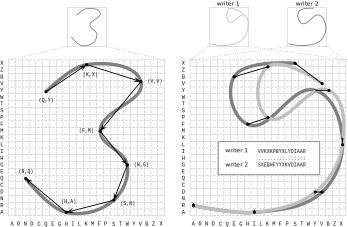
\includegraphics[width=\textwidth]{Body/Images-appc/digits.pdf}
			\caption{Projection of a digit written with
					a PDA stylus into protein space.
					Concatenating the set of
					points gives a protein sequence
					representative of the digit.
					In this case, the sequence is
					\texttt{QYKXVVFMWGSNHANQ}.%
					An alignment of nines from two
					different writers.  The boxes at
					the top show the input from each
					writer and the large grid show the
					superposition of the two handwritten
					digits.  The FastA alignment between
					the protein representations of the
					two digits is shown in the center.
				Two visualizations of the handwriting
				recognition problem.  In both cases the
				$x$ and $y$ axes are divided into 23 parts
				corresponding to the columns and rows in
				an amino acid scoring matrix.  The eight
				sampled points from the digit are cast from
				$x,y$ space into protein space by assigning
				amino acid coordinates to each point.
			}\label{fig:pda}\label{fig:pdaAlign}
		\end{figure}

		\begin{table*}[t!] 
			\centering
			\caption[fooba]{Results for the handwriting and
				speech recognition problems described
				in the text.  For each experiment,
				the misclassification is the percent of
				sequences in the unknown set for which the
				digit or letter was not predicted correctly.}
			\subtable[
				Handwriting recognition results.
			]{
\begin{tabular}{ccc}\hline\hline
Experiment & Classification & \parbox{4.8cm}{\centering \vspace{1mm}Classification in\\
Alimoglu \& Alpaydin, 1996\vspace{1mm}}  \\ \hline
1 & 97.34\%  & 97.80\% \\
2 & 99.64\% & n/a \\
%3 & 0.46\% & n/a \\
\hline\hline
\end{tabular}
} \subtable[Speech
				recognition results.
				The second column shows the
				misclassification using the clustering of
				all /ee/ sounding letters as described in the
				text.  ]{ 
\begin{tabular}{cccc}\hline\hline
Experiment & Classification & \parbox{2.5cm}{\vspace{1mm}Classification\\ with clustering\vspace{1mm}} & \parbox{4.5cm}{\centering \vspace{1mm}Classification in\\
Dietterich \& Bakiri, 1995\vspace{1mm}} \\ \hline
1 & 93.84\% & 98.91\%  & 96.73\% \\
2 & 92.61\% & 98.61\% &  n/a \\
%3 & 5.11\% & 0.71\% & n/a \\
\hline\hline
\end{tabular}
 }
			\label{table:results2}\label{table:results1}
		\end{table*}


		\begin{table*}[!b]
		\centering
		\caption[Handwriting Alignment Scoring Matrix]{The scoring matrix used for the handwriting
			and speech recognition FastA alignments.
			Each entry of the scoring matrix, $s_{ij}$, is given by $s_{ij}= 10-(|i-j|)$.
			That is, matching amino acids are given 10 ``points'', amino acids
			that are one off are given 9 points, and so on.  This matrix was used
			in place of the default scoring matrix,  Blosum50~\cite{henikoff1992aminoacid},  for FastA.
			The scoring matrix was found heuristically.  Also, a few experiments indicated that the
			alignments are relatively insensitive to permutations about the form of $s_{ij}$ given above.

		} \label{table:matrix}
		
\tiny
 \begin{tabular}{c@{\hspace{2mm}}c@{\hspace{2mm}}c@{\hspace{2mm}}c@{\hspace{2mm}}c@{\hspace{2mm}}c@{\hspace{2mm}}c@{\hspace{2mm}}c@{\hspace{2mm}}c@{\hspace{2mm}}c@{\hspace{2mm}}c@{\hspace{2mm}}c@{\hspace{2mm}}c@{\hspace{2mm}}c@{\hspace{2mm}}c@{\hspace{2mm}}c@{\hspace{2mm}}c@{\hspace{2mm}}c@{\hspace{2mm}}c@{\hspace{2mm}}c@{\hspace{2mm}}c@{\hspace{2mm}}c@{\hspace{2mm}}c@{\hspace{2mm}}c@{\hspace{2mm}}c}\hline\hline
 & A & R & N & D & C & Q & E & G & H & I & L & K & M & F & P & S & T & W & Y & V & B & Z & X\\ 
A & 10 & 9 & 8 & 7 & 6 & 5 & 4 & 3 & 2 & 1 & 0 & -1 & -2 & -3 & -4 & -5 & -6 & -7 & -8 & -9 & -10 & -11 & -12\\ 
R & 9 & 10 & 9 & 8 & 7 & 6 & 5 & 4 & 3 & 2 & 1 & 0 & -1 & -2 & -3 & -4 & -5 & -6 & -7 & -8 & -9 & -10 & -11\\ 
N & 8 & 9 & 10 & 9 & 8 & 7 & 6 & 5 & 4 & 3 & 2 & 1 & 0 & -1 & -2 & -3 & -4 & -5 & -6 & -7 & -8 & -9 & -10\\ 
D & 7 & 8 & 9 & 10 & 9 & 8 & 7 & 6 & 5 & 4 & 3 & 2 & 1 & 0 & -1 & -2 & -3 & -4 & -5 & -6 & -7 & -8 & -9\\ 
C & 6 & 7 & 8 & 9 & 10 & 9 & 8 & 7 & 6 & 5 & 4 & 3 & 2 & 1 & 0 & -1 & -2 & -3 & -4 & -5 & -6 & -7 & -8\\ 
Q & 5 & 6 & 7 & 8 & 9 & 10 & 9 & 8 & 7 & 6 & 5 & 4 & 3 & 2 & 1 & 0 & -1 & -2 & -3 & -4 & -5 & -6 & -7\\ 
E & 4 & 5 & 6 & 7 & 8 & 9 & 10 & 9 & 8 & 7 & 6 & 5 & 4 & 3 & 2 & 1 & 0 & -1 & -2 & -3 & -4 & -5 & -6\\ 
G & 3 & 4 & 5 & 6 & 7 & 8 & 9 & 10 & 9 & 8 & 7 & 6 & 5 & 4 & 3 & 2 & 1 & 0 & -1 & -2 & -3 & -4 & -5\\ 
H & 2 & 3 & 4 & 5 & 6 & 7 & 8 & 9 & 10 & 9 & 8 & 7 & 6 & 5 & 4 & 3 & 2 & 1 & 0 & -1 & -2 & -3 & -4\\ 
I & 1 & 2 & 3 & 4 & 5 & 6 & 7 & 8 & 9 & 10 & 9 & 8 & 7 & 6 & 5 & 4 & 3 & 2 & 1 & 0 & -1 & -2 & -3\\ 
L & 0 & 1 & 2 & 3 & 4 & 5 & 6 & 7 & 8 & 9 & 10 & 9 & 8 & 7 & 6 & 5 & 4 & 3 & 2 & 1 & 0 & -1 & -2\\ 
K & -1 & 0 & 1 & 2 & 3 & 4 & 5 & 6 & 7 & 8 & 9 & 10 & 9 & 8 & 7 & 6 & 5 & 4 & 3 & 2 & 1 & 0 & -1\\ 
M & -2 & -1 & 0 & 1 & 2 & 3 & 4 & 5 & 6 & 7 & 8 & 9 & 10 & 9 & 8 & 7 & 6 & 5 & 4 & 3 & 2 & 1 & 0\\ 
F & -3 & -2 & -1 & 0 & 1 & 2 & 3 & 4 & 5 & 6 & 7 & 8 & 9 & 10 & 9 & 8 & 7 & 6 & 5 & 4 & 3 & 2 & 1\\ 
P & -4 & -3 & -2 & -1 & 0 & 1 & 2 & 3 & 4 & 5 & 6 & 7 & 8 & 9 & 10 & 9 & 8 & 7 & 6 & 5 & 4 & 3 & 2\\ 
S & -5 & -4 & -3 & -2 & -1 & 0 & 1 & 2 & 3 & 4 & 5 & 6 & 7 & 8 & 9 & 10 & 9 & 8 & 7 & 6 & 5 & 4 & 3\\ 
T & -6 & -5 & -4 & -3 & -2 & -1 & 0 & 1 & 2 & 3 & 4 & 5 & 6 & 7 & 8 & 9 & 10 & 9 & 8 & 7 & 6 & 5 & 4\\ 
W & -7 & -6 & -5 & -4 & -3 & -2 & -1 & 0 & 1 & 2 & 3 & 4 & 5 & 6 & 7 & 8 & 9 & 10 & 9 & 8 & 7 & 6 & 5\\ 
Y & -8 & -7 & -6 & -5 & -4 & -3 & -2 & -1 & 0 & 1 & 2 & 3 & 4 & 5 & 6 & 7 & 8 & 9 & 10 & 9 & 8 & 7 & 6\\ 
V & -9 & -8 & -7 & -6 & -5 & -4 & -3 & -2 & -1 & 0 & 1 & 2 & 3 & 4 & 5 & 6 & 7 & 8 & 9 & 10 & 9 & 8 & 7\\ 
B & -10 & -9 & -8 & -7 & -6 & -5 & -4 & -3 & -2 & -1 & 0 & 1 & 2 & 3 & 4 & 5 & 6 & 7 & 8 & 9 & 10 & 9 & 8\\ 
Z & -11 & -10 & -9 & -8 & -7 & -6 & -5 & -4 & -3 & -2 & -1 & 0 & 1 & 2 & 3 & 4 & 5 & 6 & 7 & 8 & 9 & 10 & 9\\ 
X & -12 & -11 & -10 & -9 & -8 & -7 & -6 & -5 & -4 & -3 & -2 & -1 & 0 & 1 & 2 & 3 & 4 & 5 & 6 & 7 & 8 & 9 & 10\\ \\
\hline\hline\end{tabular}

		\end{table*}

		\begin{figure}[ptbh]
		\centering
		
\includegraphics[width=\textwidth]{Body/Images-appc/voice.pdf}
		
			%\scalebox{0.80}{
			%	\footnotesize
			%	\psset{xunit=1cm,yunit=1cm}
\readdata{\dataA}{Figures/voiceSeq1-xy.dat}
\readdata{\dataB}{Figures/voiceSeq2-xy.dat}
\begin{pspicture}(0,0)(10,10)%\showgrid
	\rput(2,9){
		\rput(-1,0){
			\psaxes[tickstyle=bottom, dy=\psyunit,Dy=1,Oy=0,Ox=0,Dx=100](0,0)(0,-1)(8,1)
		}
		\dataplot[plotstyle=line,linecolor=black,linewidth=0.1mm]{\dataA}
	}
	\rput(2,1){
		\rput(-1,0){
			\psaxes[tickstyle=bottom, dy=\psyunit,Dy=1,Oy=0,Ox=0,Dx=100](0,0)(0,-1)(8,1)
		}
		\dataplot[plotstyle=line,linecolor=black,linewidth=0.1mm]{\dataB}
	}
	\rput[l](0.4, 5.5){\normalsize \texttt{SSEMSBVFIHIMBXBMFMLFTYVMMSMTBZBTMMGTZXWTBBWICDGGG}}
	\rput[l](0.4, 5){\normalsize \texttt{:...:.......:...............:..:..::.:..:..:.....}}
	\rput[l](0.4, 4.5){\normalsize \texttt{SPQISVBWFFPVBYPPPSYZXVWSSTVBBVWTSPGTBXXYBWFIKGIIM}}
	\rput(0, 0){
		\psline[linestyle=dotted](4,2)(0.55,4.3)
		\psline[linestyle=dotted](4.4,2)(10.6,4.3)
		\psline[linestyle=dotted](4.4,2)(4.4,1)
		\psline[linestyle=dotted](4.2,2)(4.2,1)
	}
	\rput(0, 0){
		\psline[linestyle=dotted](4,8)(0.55,5.7)
		\psline[linestyle=dotted](4.4,8)(10.6,5.7)
		\psline[linestyle=dotted](4,8)(4,9)
		\psline[linestyle=dotted](4.4,8)(4.4,9)
	}
	\rput[bl](8.5, 8){Speaker 1}
	\rput[tl](8.5, 2){Speaker 2}

		
		
%	\rput(0.8,150){
%		\rotatebox{90}{ \# sequences}
%	}
%	\rput(8.5,150){
%		\rotatebox{-90}{ \# patterns}
%	}
%	\rput(5,0){
%		bootstrapping iterations
%	}


%	number LSWBBTTTTYZXBW SSEMSBVFIHIMBXBMFMLFTYVMMSMTBZBTMMGTZXWTBBWICD
%	       .............. :...:.......:...............:..:..::.:..:..:..
%	number TZXYSMFPYVVVTS SPQISVBWFFPVBYPPPSYZXVWSSTVBBVWTSPGTBXXYBWFIKG
%	250       260       270       280       290       300

%	310       320       330       340       350       360
%	number GGGCIWYFMELKKFTKPLILAAAAAAAAAADWZIHWIDDCCDNRAAAAAAAAAAAAAAAA
%	       ....................:::::::::...... ........::::::::::::::::
%	number IIMKPFIILHGDMSYTIEHEAAAAAAAAARITBTDEMGQEHCRAAAAAAAAAAAAAAAAA

\end{pspicture}

			%	\normalsize
			%}
		\caption[A Voice alignment]{
			An alignment of the spoken--letter ``X'' recorded from two different speakers.
			The plots at the top and bottom are recordings for first and second
			speakers, respectively.  The breakout in the center shows a section of the protein
			projection of each recording and the alignment generated using FastA
			as described in the text.  This example was taken from the first speech
			recognition experiment.  In this case, the bottom recording was the top
			scoring alignment against the top recording.
		}
		\label{fig:voiceAlign}
		\end{figure}

		\begin{figure}[ptbh]
		\centering
		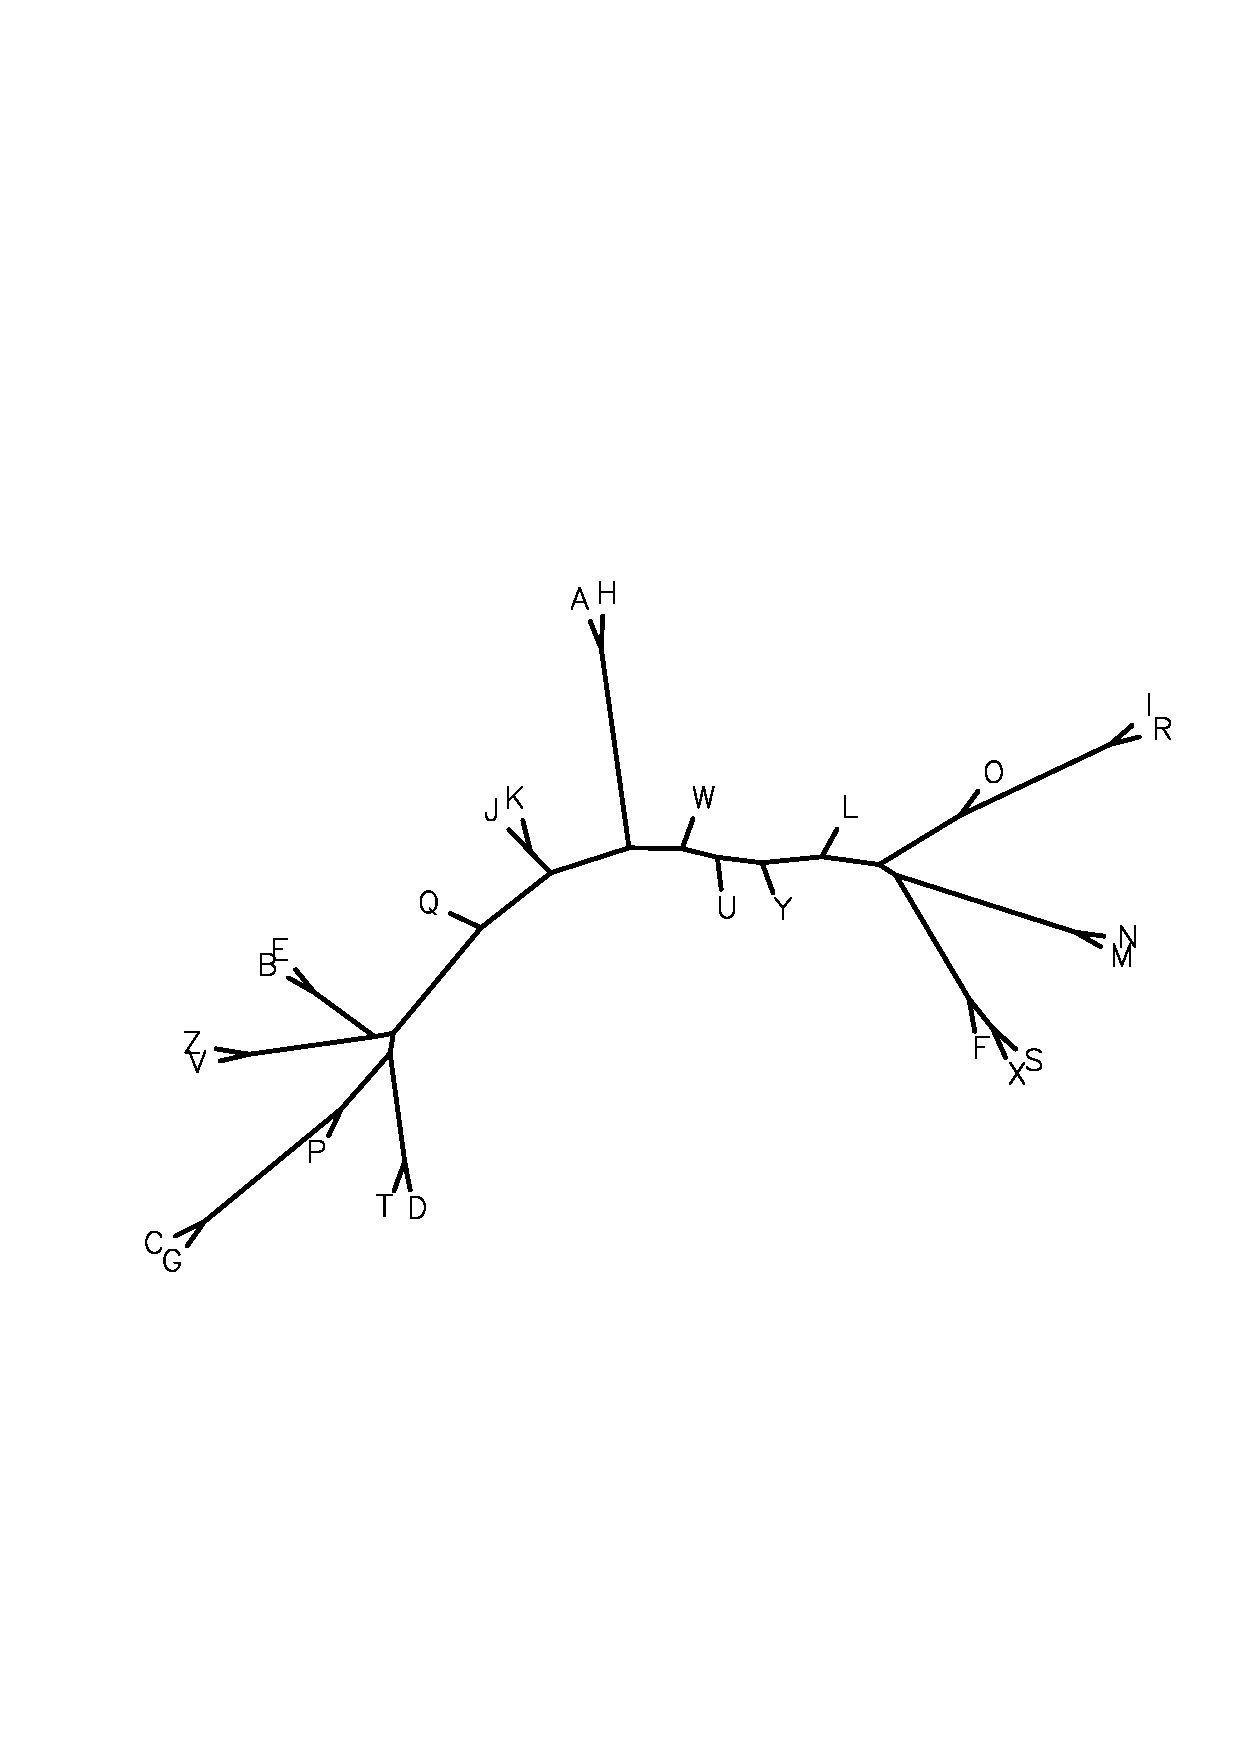
\includegraphics[width=\textwidth]{Body/Images-appc/tree.pdf}
		\caption[A PDA digit]{
			A phylogenetic tree of voice--proteins.
			This tree was created using the
			Phylip~\cite{felsenstein1989phylip} tree drawing
			program from a multiple sequence alignment of
			all 26 voice--proteins from a single speaker.
			The multiple sequence alignment was made using the
			ClustalW~\cite{higgins1992improved} alignment tool,
			with the scoring matrix in Table~\vref{table:matrix}.
			In the tree, similar sounding (homologous) letters
			are grouped near each other.  For example, all the
			letters containing the /ee/ sound [\emph{B, C, D,
			E, G, P, T, V, Z}] are clustered on the left side
			of the tree.
		} \label{fig:tree} \end{figure}



\section{System and Methods}
	\subsection{Handwriting Recognition}
		For our handwriting recognition experiments, we used
		data from Alimoglu and Alpaydin, 1996, available in the
		University of California Irvine repository of machine
		learning databases~\cite{uci1998ucirepository}.  These data
		comprised of 10992 handwritten digits between \emph{0}
		and \emph{9}, written by 44 writers with each writer
		submitting 250 digits (8 samples were discarded by the
		original authors).

		Each digit was written with a stylus pen on a touch tablet,
		which recorded the $x$ and $y$ coordinates of the pen as a
		function of time.  These data were re-sampled such that each
		written digit was represented by a series of eight $(x,y)$
		points, spaced out by a constant arc length over the path of
		the digit.  Then, for each digit, the set of $(x,y)$ points
		were scaled such that the largest axis, usually the $y$ axis,
		ranged from 0 to 1.  By dividing the number line $[0,1]$
		into 23 ``bins'' we translated each of these coordinates
		into a pair of amino acids as shown in Figure~\vref{fig:pda}.
		We concatenated these amino acid pairs to obtain a protein
		sequence representation of each digit: a ``digit--protein.''



		
	\subsection{Speech Recognition}
		For our speech recognition experiments, we used data from
		Deitterich and Bakiri, 1995, %~\cite{dietterich1995solving}
		available in the University of California Irvine repository
		of machine learning databases~\cite{uci1998ucirepository}.
		This data set consisted of 7797 recordings of individuals
		speaking one of the letters \emph{A--Z}.  A total of 150
		speakers each said every letter \emph{A--Z} twice (three
		recordings were discarded by the original authors).
		Then, each recording was processed into a set of 617
		real--valued attributes in the range $[-1,1]$.	A more
		detailed description of the database is available from
		Dietterich \& Bakiri, 1995.%~\cite{dietterich1995solving}.

		By dividing the number line $[-1,1]$ into 23 bins we translated these real numbers into a series
		of amino acids.  For example, the series ``-1.0,-0.55, 0.11, 0.65'' was translated
		to ``{\texttt{AQKY}}''.  We concatenated these amino acids to make a protein representation
		of each recording: a ``voice--protein''.


\section{Results}
	\subsection{Handwriting Recognition}

		We conducted two handwriting recognition experiments.
		In both experiments part of the digit--protein database was assumed to contain a
		``known'' set of digits that was subsequently used to annotate,
		or classify, the remaining ``unknown'' digits.	For our
		first experiment, we used for the known database containing the
		writing of 30 persons (7494 digits) and an unknown database
		with the writing of the remaining 14 persons (3498 digits).
		Using FastA, we searched each sequence from the unknown
		set in the known set and used the top scoring hits to
		annotate the unknown digits.  Searches were carried out
		using the scoring matrix shown in Table~\vref{table:matrix}
		with FastA version 3.4t11 using the default gap open and
		extension penalties, and the following options: \texttt{-p
		-Q -d0 -f-8 -g-1 -H -E1000 -b1}.  An example alignment of
		two handwritten nines from different writers is shown in
		Figure~\vref{fig:pdaAlign}.


		For our second experiment, we used 25\% (2748 digits) of our
		digit--protein database, selected randomly, as the unknown
		set and the remaining 75\% (8244 digits) as our known set.
		Alignments and annotations using FastA were performed as
		in the first experiment.

		The results of the two handwriting recognition
		experiments are shown in Table~\vref{table:results1}.
		In experiment 1, our results are about the same as
		the best k--means clustering results of Alimoglu and
		Alpaydin~\cite{alimoglu1996methods,alimoglu1997combining}.
		This experiment simulates the user--independent
		handwriting recognition problem: the handwriting of one
		group of writers was used to classify digits from a different group.
		In the user--dependent problem, experiment 2, the database
		of known handwritten digits contains samples from all the writers,
		on average.  Thus, for every unknown handwriting sample,
		there is often a close match in the database of known
		samples.  As such, the results of experiment 2 are
		significantly better than those of experiment 1 as shown
		in Table~\vref{table:results1}.



		%In contrast to k--means clustering and other common machine learning techniques for handwriting
		%recognition, there was no explicit training or learning phase of our experiments.  As such, 
		%we included experiment 3, which is a realistic approximation of the recognition problem 
		%on a tablet PC with multiple users.  The results for this experiment are considerably better than
		%experiment 2 because there are relatively more known sequences which can be used for annotating
		%the unknown sequence.

		In experiment 1, the average time for each alignment was
		0.117 seconds per unknown sequence on a 1 gHz Pentium III
		processor.  This is much shorter than the time required to
		write the digits.  Thus sequence alignment could be used
		as a ``real--time'' method for handwriting recognition.
		This high speed, together with the high accuracy for
		user--dependent recognition makes sequence alignment good
		candidate for use on a Tablet PCs, or even PDAs.

	\subsection{Speech Recognition}


		Using the voice--protein database, we conducted two
		experiments, analogous to the two handwriting recognition
		experiments described previously.  First, we used a known
		set consisting of 6238 recordings from 120 speakers and
		an unknown set with 1559 recordings from the remaining 30
		speakers.  Second, we used 25\% (1949 recordings) of the
		voice--protein database, selected randomly, as the unknown
		set and the remaining 75\% (5848 recordings) as the known
		set.  Each of the speech recognition alignments was performed
		using the same scoring matrix and FastA parameters as the
		handwriting recognition experiments.  An example alignment
		of two voice--proteins is shown in Figure~\vref{fig:voiceAlign}.


		The results of the two speech recognition experiments are shown in
		Table~\vref{table:results2}.
		Experiment 1 is compared
		to the best Error Correcting Output Code (ECOC) results of Deitterich
		and Bakiri,
		%~\cite{dietterich1995solving}
		but
		there was no comparison available for experiment 2.	
		The misclassification for experiment 1 was 6.16\%, 
		higher than the ECOC result of 3.27\%.  However, we observed that
		most of the errors were due to rhyming letters, and in particular
		all of the /ee/ sounding characters [\emph{B, C, D, E, G, P, T, V, Z}].
		This indicated that these characters were similar on a sequence level,
		so we constructed a phylogenetic tree of the sequences to study their
		relationship.

	

		A phylogenetic tree of 26 voice--proteins from a single
		speaker is shown in Figure~\vref{fig:tree}.  As the figure
		shows, the protein projections of phonetically similar
		letters tend to be homologous.	Furthermore, letters such
		as \emph{A} and \emph{H}, which have the /ay/ sound at the
		beginning, are more closely related to each other than
		they are to \emph{J} and \emph{K}, which have the /ay/
		sound at the end.  Because the /ee/ sounding letters all
		have /ee/ at the end, they are particularly difficult
		to distinguish from each other.  These letters account
		for a disproportionate majority of the errors in our two
		experiments.  By clustering these letters together such that
		they are considered the same for classification purposes,
		the error in experiment 1 was reduced to 1.09\%.  If the
		original error was evenly distributed between the classes,
		the error would have been reduced only to about 5.5\%.
		This suggests that, although string alignment performs
		poorly for /ee/ sounding characters, it performs well for
		all other characters.


\section{Conclusions}
		This work showed that sequence alignment can be a powerful
		classification tool for problems outside the domain
		of bioinformatics.  In both the handwriting and speech
		recognition problems, we projected real--valued data into
		strings of amino acids and used FastA as a classification
		tool, in a manner analogous to protein annotation.  In the
		case of handwriting recognition, we showed that sequence
		alignment is a viable alternative to traditional methods,
		such as k--means clustering, and is fast enough to be used
		as a real--time recognition method.


		There are many ways to improve upon the results we presented here.
		First, we did not have any explicit training phase for either set of experiments.
		However, there are at least two sequence alignment parameters which can
		be trained: the gap open and extension penalties, and the scoring matrix.
		The optimization of these parameters for protein annotation is well documented
		~\cite{henikoff1993performance,altschul1991amino,henikoff1992aminoacid,dayhoff1979amodel,vogt1995assessment,henikoff2000amino}
		and would be similar for alternative sequence alignment applications such
		as handwriting recognition.  Second, intelligent projection of data
		into strings can greatly improve results.  Here, we used bins of equal
		size to partition the real--valued data into amino acids; however, bins
		of unequal size may improve the resolution between closely related sequences
		and improve classification.  Finally, more customizable sequence alignment tools
		would be very useful.  These tools should take an arbitrary alphabet (Blast
		and FastA are restricted to 23 amino acids) and a user--defined scoring
		matrix (FastA allows user--defined matrices, but Blast does not).

		The potential applications of sequence alignment tools
		outside of bioinformatics are boundless.  Tools such as Blast
		and FastA can be used to quickly classify or search through
		any data that can be projected into a string of characters.
		Of course, these methods will work best with data that is
		of a low dimension.  Our experiments with more complex data
		data, such as color images, suggest that how the data are
		projected into a string is very important with large number
		of dimensions.	However, for simple types of data, such
		as customer purchase histories, black and white images, or
		Internet chat transcripts, we have been able to use sequence
		alignment as a quick and effective classification tool.

